\subsubsection*{Registrieungsschlüssel \faKey}

Über den Button \jinline|Edit| kann der Administrator dem Registrierungsschlüssel ändern können, sodass im Falle eines \emph{Leaks} des Registierungsschlüssels ein Registrieren neuer Benutzer nicht mehr möglich ist (siehe Abb. \vref{fig:AdminEditRegKeyImplement}). 
Über den Button \jinline|Show|\xspace kann er den aktuellen Registierungsschlüssel auslesen, im Falle, dass er diesen nicht mehr kennt. 

\begin{figure}[hp]
	\centering
	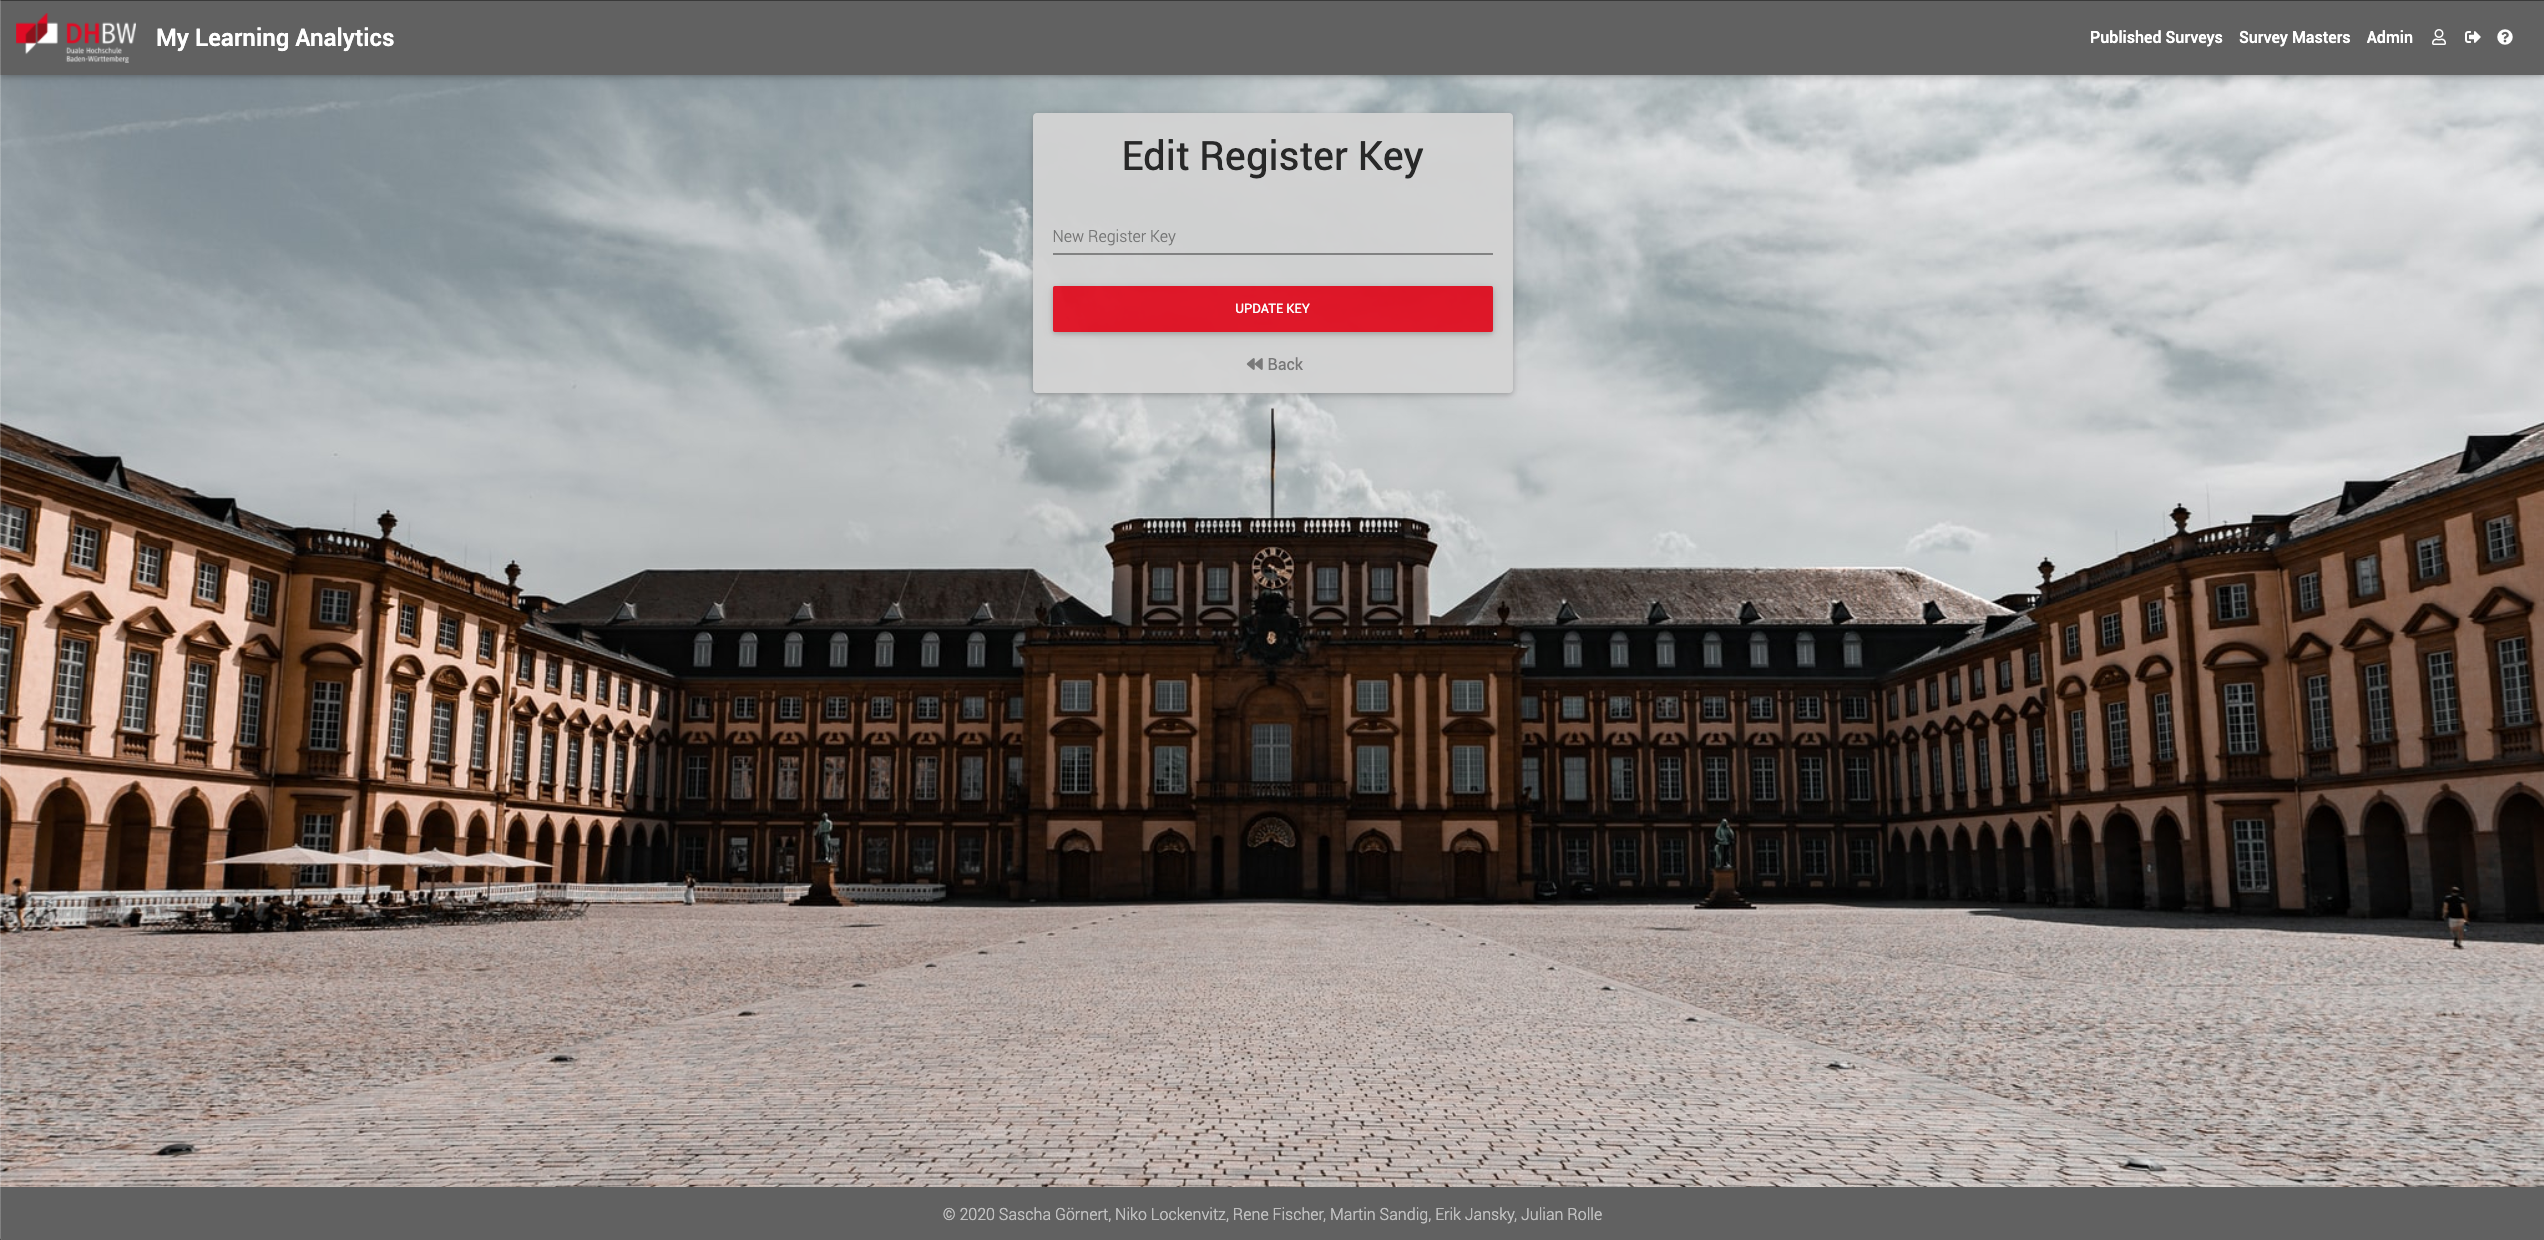
\includegraphics[width=0.95\textwidth, keepaspectratio]{img/client/EditSurveyMasterKey.png}
	\captionsetup{justification=centering, format=plain}
	\caption[\acf{UI}: Setzen eines neuen Registierungsschlüssels]{\acf{UI}: Setzen eines neuen Registierungsschlüssels \\ \quelleScreenshot}
	\label{fig:AdminEditRegKeyImplement}
\end{figure}